\documentclass[a4paper]{jarticle}
\usepackage{graphicx}
\begin{document}

研究室のプリンタに合わせた

\begin{figure}
  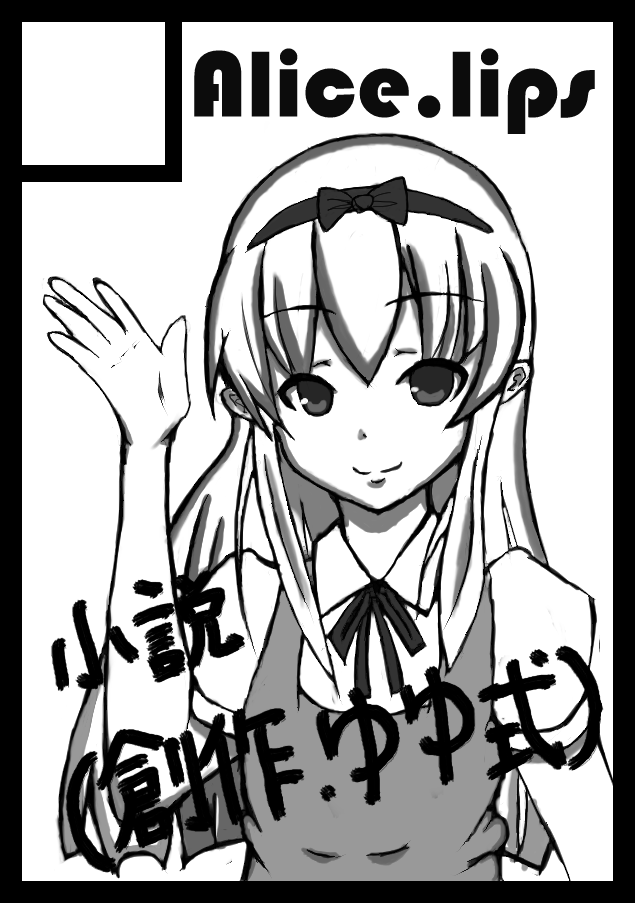
\includegraphics[width=37mm,bb=0 0 600 853]{alice.png}
  \hfill
  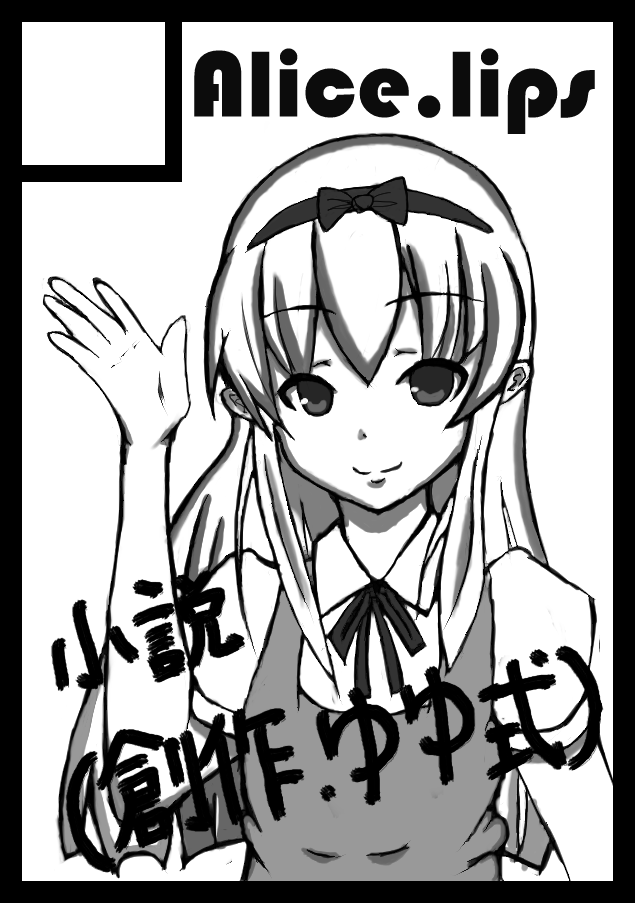
\includegraphics[width=37mm,bb=0 0 600 853]{alice.png}
  \caption{width=37}
\end{figure}

\begin{figure}
  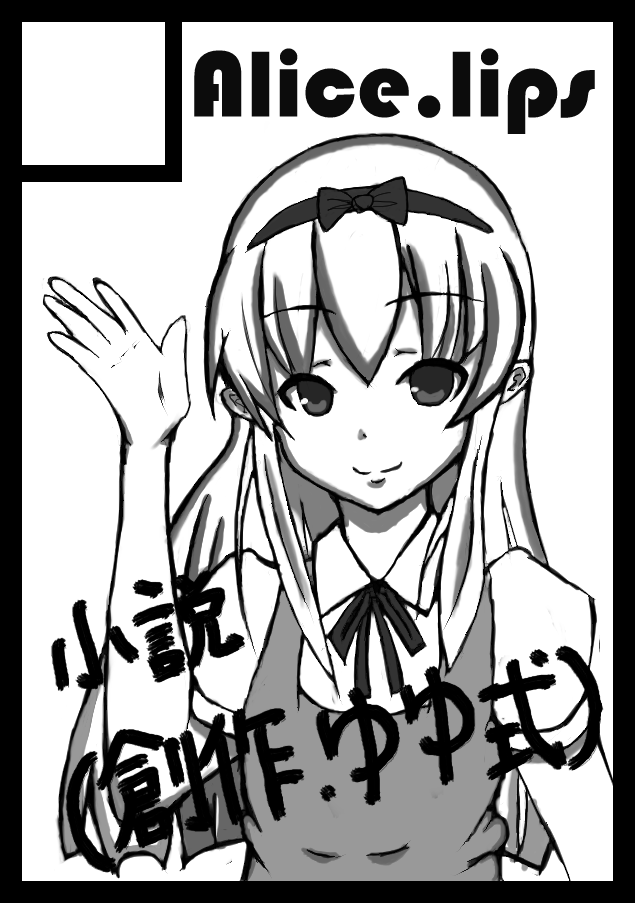
\includegraphics[width=38mm,bb=0 0 600 853]{alice.png}
  \hfill
  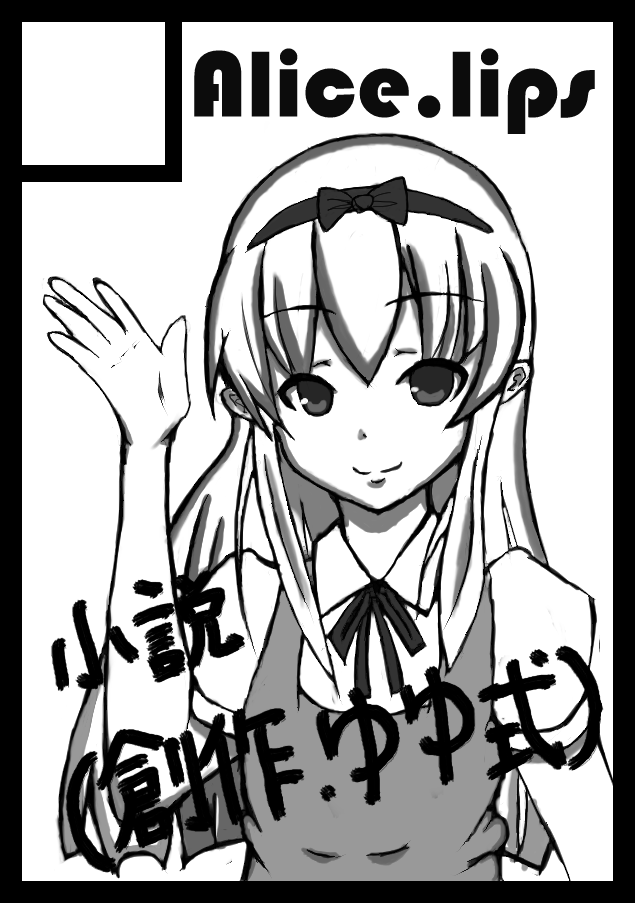
\includegraphics[width=38mm,bb=0 0 600 853]{alice.png}
  \caption{width=38}
\end{figure}

\end{document}
